\section{Spezialthemen}

\subsection{XXE File Inclusion}
Unter dem Begriff ist eine Attacke über das \textit{XML External Entity Processing} möglich. Dabei können externe Daten, wie z.B. lokale Dateien, in das XML inkludiert werden. Bei der Verarbeitung solcher Inclusions, welche im DTD angegeben sind, fügt sie der Parser in die angegebenen Stelle ein.\\

\textbf{Lösung:} Deaktivierung des Features für DTDs (External Entities) beim Parser.

\begin{lstlisting}[language=XML, caption=Beispiel der XXE]
<?xml version="1.0" encoding="ISO-8859-1"?>
<!DOCTYPE foo [  
  <!ELEMENT foo ANY >
  <!ENTITY xxe SYSTEM "file:///etc/passwd" >]>
<foo>&xxe;</foo>
\end{lstlisting}

\subsection{URL-Redirection Attack}
URL-Redirection wird häufig im Zusammenhang mit Phishing verwendet, mit dem Ziel, eine Session übernehmen zu können. Dazu wird dem Opfer ein Link untergeschoben, der auf den ersten Blick vertrauenswürdig aussieht. In Wirklichkeit enthält dieser jedoch einen Redirect auf eine Landing-Page des Hackers. Klickt das Opfer auf diesen Link, so wird normal das Login-Formular der vertrauenswürdigen Website geladen. Gibt das Opfer nun seine Credentials ein, werden diese auf Korrektheit geprüft und es wird auf die Landing-Page des Hackers weitergeleitet. Dort erscheint eine präparierte Fehlermeldung, dass die Anmeldung fehlgeschlagen sei und der Benutzer meldet sich erneut an. Diesmal erhält allerdings der Hacker die Anmeldeinformationen und dem Opfer erscheint eine Meldung, dass die gewünschte Seite nicht mehr erreichbar ist. \\

\textbf{Beispiel:} http://www.example.com/login?redirect=http://www.hack.er \\

\textbf{Lösung:}
\begin{easylist}
	& Inputvalidierung
	&& Parameter die Redirect URLS enthalten validieren
	&& Prüfen ob URL wirklich zur Seite gehört
	& Lookup Tables
	&& Erstellen von Mappings zwischen Parameter und URL
	&& redirect=1
	&& redirect=acc
\end{easylist} 

\subsection{HTTP Request Smuggling / Splitting}
HTTP Request Smuggling Attacken werden benutzt, um beispielsweise WAFs zu umgehen. Dabei wird die Schwachstelle ausgenutzt, dass verschiedene Sicherheitssysteme HTTP Requests unterschiedlich interpretieren. Beispielsweise kann mit CR/LF (Carriage Return / Line Feed) erreicht werden, dass ein einzelner Request aus zwei unabhängigen Requests besteht. Die WAF erkennt nur den ersten, der dahinter verborgene Webserver antwortet jedoch auf beide Requests. Somit können Informationen, die eigentlich nur zwischen WAF und Webserver sichtbar sein sollten, nach "'aussen"' gelangen. Beispielsweise ein Cookie welches zwischen WAF und Webserver einen User authentifiziert.\\

Oftmals werden die Felder \textit{Location} und \textit{Set-Cookie} als Ziel verwendet. Übliche Escape-Sequenzen sind: \lstinline|%0a %0d %0a%0d %0d%0a|

\begin{lstlisting}[language={},caption=Beispiel eines präparierten Requests zur Umgehung einer Pre-Authentication]
username=hacker10&url=%2Fsecure%0aSet-Cookie:LOGON=OK; %0aSet-Cookie:MOD_BUT_Username=admin;&lang=EN&password=compass
\end{lstlisting}

\textbf{Lösung:}
\begin{easylist}
	& Web Application Firewalls verwenden, die nicht verwundbar gegen HTTP Request Smuggling sind.
	& Strenges Sessionmanagement verwenden, z.B Session nach jedem Request terminieren.
	& Aktivieren von Strict Parsing beim Webserver, z.B. Apache.
\end{easylist}

\subsection{Mass Assignment Vulnerability}
Software Frameworks erlauben Entwicklern manchmal HTTP Request Parameter automatisch auf Variablen oder Objekte im Programm Code zu binden. Angreifer können so evtl. nicht vorgesehene Parameter setzen und dadurch möglicherweise das Verhalten einer Methode beeinflussen.\\

\textbf{Beispiel}: Das Autobinding in ASP.NET MVC ist anfällig auf diese Angriffe.
\begin{figure}[H]
	\centering
	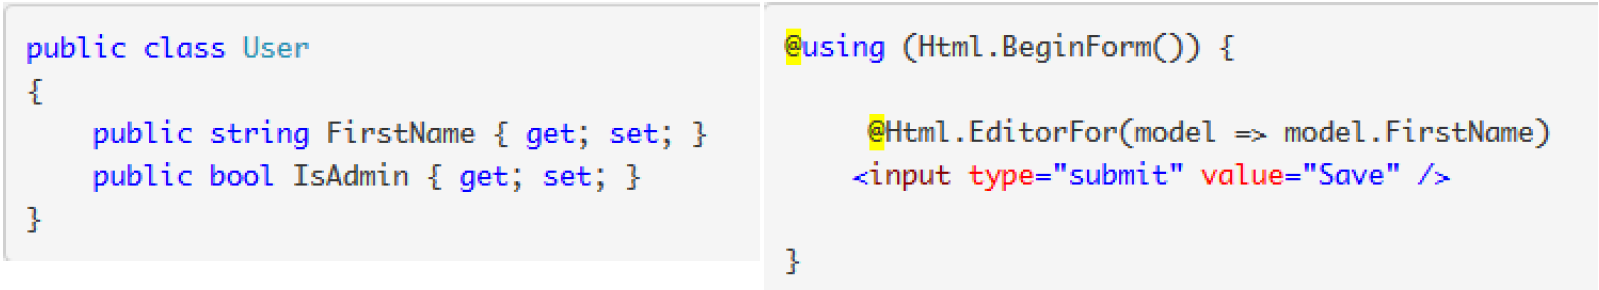
\includegraphics[width=\textwidth]{./img/mass-assignment-vulnerability}
	\caption{Verwundbarer Beispielcode in ASP.NET MVC}
\end{figure}
\begin{lstlisting}[language={},caption=Beispiel eines präparierten Requests zum Setzen eines nicht vorgesehenen Parameters]
POST /addUser
FirstName=Scott&isAdmin=true
\end{lstlisting}

\textbf{Lösung: Es genügt nicht, ein IsAdmin Flag aus dem Editform wegzulassen.}

\begin{description}
	\item[Whitelist] alle benötigten Parameter explizit binden
	\item[Blacklist] alle nicht benötigten Parameter explizit ausschliessen
	\item[Strongly Typed] eine Interface Definition für ein spezifisches Model der benötigten Parameter
	\item[ReadOnly] in ASP.NET MVC gibt es ein ReadOnly Flag für Model Attribute
	\item[Architektonischer Ansatz] Es gibt hier mehrere Ansätze, einer davon ist der Einsatz von DTOs (Data Transfer Objects).
\end{description}

\subsection{Advanced Persistent Threat - APT}
Ein Advanced Persistent Threat (\textit{fortgeschrittene, andauernde Bedrohung}) beschreibt einen komplexen, zielgerichteten und effektiven Angriff auf kritische IT-Infrastrukturen und vertrauliche Daten von Behörden und Unternehmen, welche aufgrund ihres Technologievorsprungs potenzielle Opfer darstellen.\\
Die Angreifer gehen sehr zielgerichtet vor und nehmen einen grossen Aufwand auf sich. Das Ziel eines APT ist es, möglichst lange handlungsfähig zu bleiben, um über einen längeren Zeitraum sensible Informationen auszuspähen oder anderweitig Schaden anzurichten.\\
\textbf{Abwehrstrategien:}
\begin{easylist}
	& Logging
	& Lookup Services (Blacklists, Malware Hashes, OpenIOC, IP Reputation Lists)
\end{easylist}
